\documentclass[14pt, a4paper]{article}
\usepackage{minitoc}
\usepackage[left=3.00cm, right=2.5cm, top=2.00cm, bottom=2.00cm]{geometry}
\usepackage{amsmath}
\usepackage{amssymb}
\usepackage{amsthm}
\usepackage{mathtools}
\usepackage{graphicx}
\usepackage{algpseudocode}
\usepackage{algorithm}
\usepackage{blindtext}
\usepackage{setspace}
\usepackage[utf8]{inputenc}
\usepackage[utf8]{vietnam}
\usepackage[center]{caption}
\usepackage{fancyhdr} % header, footer
\usepackage{hyperref} % loại bỏ border với mục lục và công thức
\pagestyle{fancy}
%\usepackage[style=numeric,sortcites]{biblatex}
%\addbibresource{ref.bib}
%\usepackage[numbers]{natbib}
\usepackage{indentfirst}
\usepackage[natbib,backend=biber,style=ieee, sorting=ynt]{biblatex}
\bibliography{ref.bib}

\graphicspath{{./figures/}}

%\renewbibmacro*{cite}{%
%  \printtext[bibhyperref]{%
%    \printfield{prefixnumber}%
%    \printfield{labelnumber}%
%    \ifbool{bbx:subentry}%
%      {\printfield{entrysetcount}}%
%   \ifnumequal{\value{citecount}}{\value{citetotal}-1}%
%       {\gdef\multicitedelim{\addspace\bibstring{and}\space}}%
%       {\gdef\multicitedelim{\addcomma\space}}%
%    }%
%}

\hypersetup{
    colorlinks=false,
    pdfborder={0 0 0},
}

\title{Tiểu luận phương pháp số cho đại số tuyến tính}

\author{Nguyễn Chí Thanh}

%\date{24-04-2022}
\fancyhf{}
\rhead{\textbf{Học viên thực hiện: Nguyễn Chí Thanh}}
\lhead{\textbf{GVHD: TS. Nguyễn Trung Hiếu}}
\rfoot{\thepage}
\lfoot{\textbf{Phương pháp số cho đại số tuyến tính}}
\renewcommand{\headrulewidth}{0.4pt}
\renewcommand{\footrulewidth}{0.4pt}

\numberwithin{equation}{section}
\numberwithin{algorithm}{section}
\numberwithin{figure}{section}

\setlength{\parindent}{0.5cm}

\setcounter{secnumdepth}{3} % Cho phép subsubsection trong report
\setcounter{tocdepth}{3} % Chèn subsubsection vào bảng mục lục

\newtheorem{dl}{Định lý}
\newtheorem{md}{Mệnh đề}
\newtheorem{bd}{Bổ đề}

\numberwithin{dl}{section}
\numberwithin{md}{section}
\numberwithin{bd}{section}

\doublespacing
\begin{document}

%\begin{titlepage}
%
%    \newcommand{\HRule}{\rule{\linewidth}{0.5mm}} % Defines a new command for the horizontal lines, change thickness here
%    
%    \center % Center everything on the page
%     
%    %----------------------------------------------------------------------------------------
%    %	HEADING SECTIONS
%    %----------------------------------------------------------------------------------------
%    \textsc{\LARGE Đại học Quốc Gia Hà Nội}\\[0.5cm]
%    \textsc{\LARGE Đại học Khoa học tự nhiên}\\[0.5cm] % Name of your university/college
%    \textsc{\LARGE Khoa Toán - Cơ - Tin học}\\[0.5cm]
%
%    
\includegraphics[scale=0.2]{HUS-logo.jpg}\\[0.5cm]
%
%    \textsc{\Large Chuyên ngành: Khoa học dữ liệu}\\[0.5cm] % Major heading such as course name
%
%    
%    %----------------------------------------------------------------------------------------
%    %	TITLE SECTION
%    %----------------------------------------------------------------------------------------
%    
%    \HRule \\[0.4cm]
%    { \huge \bfseries Tiểu luận môn học}\\[0.4cm] % Title of your document
%    \HRule \\[1.5cm]
%
%    \textsc{\Large Môn học: Phương pháp số cho đại số tuyến tính }\\[1.5cm] % Minor heading such as course title
%
%
%    \textsc{\Large Đề tài: Tìm hiểu thuật toán MINRES.\\So sánh thuật toán GMRES và thuật toán MINRES }\\[1.5cm]
%     
%
%    %----------------------------------------------------------------------------------------
%    %	AUTHOR SECTION
%    %----------------------------------------------------------------------------------------
%    \begin{minipage}{0.4\textwidth}
%        \begin{flushleft} \Large
%        \emph{Giảng viên hướng dẫn:} \\
%        TS. Nguyễn Trung Hiếu % Supervisor's Name
%        \end{flushleft}
%    \end{minipage}\\[1cm]
%
%    \begin{minipage}{0.4\textwidth}
%    \begin{flushleft} \Large
%    \emph{Học viên thực hiện:}\\
%    Nguyễn Chí Thanh \\
%    MSHV: 21007925 \\ % Your name
%    Lớp: Khoa học dữ liệu - K4
%    \end{flushleft}
%    \end{minipage}
%    
%    
%    % If you don't want a supervisor, uncomment the two lines below and remove the section above
%    %\Large \emph{Author:}\\
%    %John \textsc{Smith}\\[3cm] % Your name
%    
%    %----------------------------------------------------------------------------------------
%    %	DATE SECTION
%    %----------------------------------------------------------------------------------------
%    
%    % I don't want day because it is English
%    % {\large \today}\\[2cm] % Date, change the \today to a set date if you want to be precise
%    
%    %----------------------------------------------------------------------------------------
%    %	LOGO SECTION
%    %----------------------------------------------------------------------------------------
%    
%    %\includegraphics{logo/rsz_3logo-khtn.png}\\[1cm] % Include a department/university logo - this will require the graphicx package
%     
%    %----------------------------------------------------------------------------------------
%    
%    \vfill % Fill the rest of the page with whitespace
%    
%\end{titlepage}

\cleardoublepage
\pagenumbering{gobble}
\tableofcontents
\newpage
\listoffigures
\cleardoublepage
\pagenumbering{arabic}

%\maketitle

\newpage

\nocite{*}

\begin{center}
\section*{LỜI MỞ ĐẦU}
\end{center}
\addcontentsline{toc}{section}{{\bf LỜI MỞ ĐẦU}\rm}

\newpage

\section{Tổng quan về các phương pháp lặp trên không gian con Krylov}

Các phương pháp trên không gian con Krylov là một nhóm quan trọng trong việc giải các hệ phương trình. Ta xét một phép biến đổi tuyến tính dưới dạng một hộp đen:

\begin{equation}
    x \rightarrow \boxed{\mathrm{black} \thickspace \mathrm{box}} \rightarrow Ax
\end{equation}

Chúng ta muốn xây dựng một phương pháp lặp sao cho $x_n \rightarrow x$ với $Ax=b$ khi $n \rightarrow \infty$. Gọi $x_n \in \mathcal{K}_n$ với $\mathcal{K}_n$ là không gian con Krylov thứ n $\mathcal{K}_n=\mathrm{span} \lbrace b, Ab, A^2b, \dots, A^{n-1}b \rbrace$
Các đặc điểm của không gian con Krylov:
\begin{itemize}
    \item Ta có thể xây dựng $\mathcal{K}_n$ như một hộp đen
    \item $\mathcal{K}_n \subseteq \mathcal{K}_{n+1}$
    \item Giả sử $p^n(A)$ là một đa thức của ma trận $A$. Bất kỳ một tổ hợp tuyến tính của các vector $b, Ab, \dots$ cũng bằng $p^n(A)$ nhân với $b$, $\lVert b - Ax \rVert_2^2 = \lVert p^n(A)b \rVert_2^2$
\end{itemize}

Ta xét ma trận Krylov, $K_n = \begin{bmatrix} b, Ab, A^2b, \dots, A^{n-1}b \end{bmatrix}$. Đây là một ma trận điều kiện tồi. Vì khi $n$ càng lớn, vector $A^nb$ tiến gần đến bội của một vector riêng của ma trận $A$, làm cho ma trận $K_n$ rất gần với một ma trận kỳ dị. Vì vậy ta cần làm việc với một hệ sơ sở trực chuẩn.

Với ma trận $A$ có kích thước $m \times m$, ta có thể tính một ma trận trực giao $Q$ và một ma trận Hessenberg $H$ có dạng một ma trận tam giác trên và một đường chéo phụ:

\begin{equation} \label{eq:AQHQ}
    A = QHQ^T
\end{equation}

$Q_n=\begin{bmatrix} q_1, q_2, \dots, q_n \end{bmatrix}$ là $n$ cột đầu của ma trận $Q$:

\begin{equation} \label{eq:Hessenberg_matrix}
    \widetilde{H}_n = \begin{bmatrix} h_{1,1} & h_{1, 2} & \dots & h_{1, n} \\
    h_{2, 1} & h_{2, 2} & \dots & h_{2, n} \\
    0 & h_{3, 2} & \dots  & h_{3, n} \\
    \vdots & \space & \space & \vdots \\
    0 & \dots & h_{n, n-1} & h_{n, n} \\
    0 & 0 & \dots & h_{n+1, n}\end{bmatrix}
\end{equation}

$\widetilde{H}_n$ là ma trận tam giác trên và một đường chéo phụ kích thước $(n+1)\times n$ với:

\begin{equation} \label{eq:A_projection}
    AQ_n = Q_{n+1}\widetilde{H}_n
\end{equation}

\begin{equation} \label{eq:recurrence_term}
    Aq_n = h_{1, n}q_1 + h_{2, n}q_2 + \dots + h_{n, n}q_n + h_{n+1, n}q_{n+1}
\end{equation}


\subsection{Thuật toán lặp Arnoldi}


\begin{algorithm}
    \caption{Thuật toán Arnoldi}\label{alg:Arnoldi}
    \begin{algorithmic}
        \State {Cho ma trận $A, b$}
        \State {$q_1 \leftarrow b/\lVert b \rVert$}
        \For {$n = 1,2,3,\dots$}
            \State $v \leftarrow Aq_n$
            \For {$j=1$ to $n$}
                \State $h_{j,n} \leftarrow q_j^T v$
                \State $v \leftarrow v - h_{j,n}q_j$
            \EndFor
            \State $h_{n+1,n} \leftarrow \lVert v \rVert$
            \State $q_{n+1} \leftarrow v/h_{n+1,n}$
        \EndFor
    \end{algorithmic}
\end{algorithm}

Công thức \ref{eq:recurrence_term} là công thức truy hồi $n+1$ tham số cho vector $q_{n+1}$. Ma trận \ref{eq:Hessenberg_matrix} thu được từ quá trình trực chuẩn hóa Gram-Schmidt. Quá trình này được gọi là thuật toán Arnoldi được miêu tả ở thuật toán \ref{alg:Arnoldi}. $Q_n=\begin{bmatrix} q_1, q_2, \dots, q_n \end{bmatrix}$ là cơ sở trực chuẩn của không gian con Krylov thứ n $\mathcal{K}_n$.
Nhân cả 2 vế công thức \ref{eq:A_projection} với $Q_n^T$ ta được:

\begin{equation}
    Q_n^TAQ_n=Q_n^TQ_{n+1}\widetilde{H}_n \\
    \Rightarrow Q_n^TQ_{n+1}\widetilde{H}_n = \begin{bmatrix}
        q_1^T \\ q_2^T \\ \vdots \\ q_n^T
    \end{bmatrix} \begin{bmatrix} q_1, q_2, \dots, q_n, q_{n+1} \end{bmatrix}
    \begin{bmatrix} H_n \\ h_{n+1,n}e_n^T \end{bmatrix}=\begin{bmatrix} I & 0 \end{bmatrix} \begin{bmatrix} H_n \\ h_{n+1,n}e_n^T \end{bmatrix}=H_n
\end{equation}

$H_n$ là ma trận thu được bằng cách lấy $n$ hàng đầu của ma trận $\widetilde{H}_n$. $H_n$ có thể được giải thích là biểu diễn trong hệ cơ sở $\lbrace q_1, q_2, \dots, q_n \rbrace$ của phép chiếu trực giao của ma trận $A$ lên $\mathcal{K}_n$, giới hạn ánh xạ $A: \mathbb{C}^m \mapsto \mathbb{C}^m$ sang $H_n: \mathcal{K}_n \mapsto \mathcal{K}_n$. Phép chiếu này được gọi là phép chiếu Rayleigh-Ritz.
Các thành phần nằm trên đường chéo của ma trận $H_n$ chính là các thương số Rayleigh tương ứng với vector $q_j$. Với thương số Rayleigh được tính bằng công thức:

\begin{equation}
    r(x) = \dfrac{x^T A x }{x^T x}
\end{equation}

Các giá trị riêng của ma trận $H_n$ được gọi là ước lượng giá trị riêng Arnoldi (tại bước $n$) hoặc các giá trị Ritz (tương ứng với $\mathcal{K}_n$) của A. Một vài số trong những số này có thể xấp xỉ bằng một vài trong những giá trị riêng của ma trận $A$ ngay cả khi $n$ nhỏ hơn rất nhiều so với $m$

Để sử dụng thuật toán lặp Arnoldi để ước lượng các giá trị riêng, ta tính giá trị riêng của $H_n$ tại bước thứ $n$. Nếu $m=n$, các giá trị Ritz là các giá trị riêng của ma trận $A$. Nói chung, nếu $n \ll m$, chỉ một số ít giá trị riêng được ước lượng. Thường các giá trị riêng có giá trị gần vùng biên của phổ (tập các giá trị riêng) sẽ được hội tụ đầu tiên.

Trong nhiều ứng dụng thực tế, các giá trị tại khu vực gần biên của phổ được quan tâm chủ yếu:

\begin{itemize}
    \item Phân tích tích ổn định thường yêu cầu ước lượng bán kính phổ
    \item Phân tích thành phần chính thường yêu cầu ước lượng giá trị riêng lớn nhất và các vector riêng tương ứng của ma trận $A^T A$
\end{itemize}

Nếu $A$ có $m$ giá trị riêng phân biệt, thuật toán lặp Arnoldi tìm được tất cả các giá trị riêng này sau $m$ bước. Trong một số trường hợp cụ thể, tốc độ hội tụ trong việc ước lượng các giá trị riêng của thuật toán lặp Arnoldi mang tính hình học (tuyến tính, hàm mũ, ...).

Một số những đặc tính bất biến của thuật toán lặp Arnoldi được nêu ở trong định lý \ref{dl:Arnoldi_Properties}

\begin{dl} \label{dl:Arnoldi_Properties}
    Một thuật toán lặp Arnoldi áp dụng cho một ma trận $A \in \mathbb{R}^{m \times m}$ thỏa mãn các tính chất sau:
    \begin{itemize}
        \item \textbf{Bất biến tịnh tiến:} Nếu ma trận $A$ thay đổi thành $A + \sigma I $ với một số $\sigma \in \mathbb{R}$, và $b$ không đổi thì các giá trị Ritz $\lbrace \theta_j \rbrace$ thay đổi thành $\lbrace \theta_j + \sigma \rbrace$
        \item \textbf{Bất biến co dãn:} Nếu ma trận $A$ thay đổi thành $\sigma A$ với một số $\sigma \in \mathbb{R}$ và $b$ không đổi thì $\lbrace \theta_j \rbrace$ thành $\lbrace \sigma \theta_j \rbrace$
        \item \textbf{Bất biến dưới phép biến đổi tương đương trực giao:} Nếu ma trận $A$ thay đổi thành $UAU^T$ với một ma trận $U$ trực giao bất kỳ, $b$ thay đổi thành $Ub$ thì $\lbrace \theta_j \rbrace$ không đổi
    \end{itemize}
    Trong cả ba trường hợp trên, các vector Ritz $Q_n y_n$ tương ứng với vector riêng $y_j$ của ma trận $H_n$ không đổi dưới bất kỳ phép biến đổi nào đã được nêu trên.
\end{dl}

Một trường hợp đặc biệt, trong quá trình thực hiện thuật toán Arnoldi, tại một bước $n$ nào đó khi tính $v \leftarrow v - h_{j,n}q_j$, nếu thu được $v=0$ ta có thể dừng luôn thuật toán Arnoldi vì không gian con Krylov đã mở rộng đến cực đại, các điều sau đồng thời xảy ra:


\begin{itemize}
    \item $A\mathcal{K}_n \subseteq  \mathcal{K}_n$
    \item $\mathcal{K}_n=\mathcal{K}_{n+1}=\mathcal{K}_{n+2}=\dots$
    \item Từng giá trị riêng của$ H_n$ là giá trị riêng của $A$
    \item Nếu ma trận $A$ là ma trận không kỳ dị, nghiệm chính xác của phương trình $Ax=b$ nằm trong $\mathcal{K}_n$
\end{itemize}


Thuật toán lặp Arnoldi thuận tiện cho việc xây dựng cơ sở cho không gian con Krylov $\mathcal{K}_{n+1}$ từ cơ sở $\mathcal{K}_n$, mỗi bước này tạo thêm một vector mới $q_{n+1}$ và tránh việc sử dụng vector $A^n b$

Thuật toán Arnoldi được sử dụng trong các trường hợp:
\begin{itemize}
    \item Là cơ sở cho các thuật toán lặp giải hệ phương trình (GMRES, ...).
    \item Kỹ thuật tính giá trị riêng của ma trận không đối xứng.
\end{itemize}

\subsection{Thuật toán lặp Lanczos}


Nếu $A$ là ma trận đối xứng thì ma trận $\widetilde{H}_n$ trở thành ma trận ba đường chéo $\widetilde{T}_n$ có dạng:

\begin{equation} \label{eq:Trigonal_Matrix}
    \widetilde{T}_n = \begin{bmatrix}
        \alpha_1 & \beta_1 & \space & \space & \space \\
        \beta_1 & \alpha_2 & \beta_1 & \space & \space \\
        \space & \beta_2 & \alpha_3 & \ddots & \space \\
        \space & \space & \ddots & \ddots & \beta_{k-1} \\
        \space & \space & \space & \beta_{k-1} & \alpha_k \\
        \space & \space & \space & \space & \beta_{n}
    \end{bmatrix}
\end{equation}

Ma trận $\widetilde{T}_n$ thu được từ thuật toán Lanczos được miêu tả ở thuật toán \ref{alg:Lanczos}
Với:

\begin{equation} \label{eq:Three-term-recurrence}
    AQ_n = Q_{n+1}\widetilde{T}_n \Rightarrow Q_n^TAQ_n = Q_n^TQ_{n+1}\widetilde{T}_n=\begin{bmatrix}
        q_1^T \\ q_2^T \\ \vdots \\ q_n^T
    \end{bmatrix} \begin{bmatrix} q_1, q_2, \dots, q_n, q_{n+1} \end{bmatrix}\begin{bmatrix}
        T_n \\ \beta_n e_n^T
    \end{bmatrix}=\begin{bmatrix}
        I & 0
    \end{bmatrix} \begin{bmatrix}
        T_n \\ \beta_n e_n^T
    \end{bmatrix}=T_n
\end{equation}

$T_n$ là ma trận thu được bằng cách lấy $n$ hàng đầu của ma trận $\widetilde{T}_n$. 
Ma trận $T_n$ về mặt hình thức còn được gọi là ma trận truy hồi ba tham số.

\begin{algorithm}
    \caption{Thuật toán Lanczos}\label{alg:Lanczos}
    \begin{algorithmic}
        \State {Cho ma trận $A$ đối xứng, $b$}
        \State {$\beta_0 \leftarrow 0$}
        \State {$q_0 \leftarrow 0$}
        \State {$q_1 \leftarrow b/\lVert b \rVert$}
        \For {$n=1,2,3,\dots$}
            \State $v \leftarrow Aq_n$
            \State $\alpha_n=q_n^Tv$
            \State $v \leftarrow v - \beta_{n-1}q_{n-1} - \alpha_n q_n$
            \State $\beta_n \leftarrow \lVert v \rVert$
            \State $q_{n+1}=v/\beta_n$
        \EndFor
    \end{algorithmic}
\end{algorithm}

Từ thuật toán \ref{alg:Lanczos}, ta nhận thấy mỗi bước của thuật toán Lanczos, bao gồm một phép nhân ma trận, một phép tích vô hướng và hai phép trừ vector, ít hơn so với thuật toán Arnoldi (1 phép nhân ma trận, $n$ phép tích vô hướng và $n$ phép trừ vector)
Thuật toán đặc biệt hiệu quả cho những ma trận thưa. Trong thực tế, thuật toán lặp Lanczos hay được sử dụng để tính các giá trị riêng của các ma trận đối xứng có kích thước lớn.

Cũng giống như thuật toán lặp Arnoldi, thuật toán lặp Lanczos cũng rất hữu ích và hay được sử dụng cho các bài toán:

\begin{itemize}
    \item Cơ sở cho các thuật toán lặp (ví dụ MINRES, Gradient liên hợp)
    \item Một kỹ thuật dùng để ước lượng giá trị riêng của các ma trận đối xứng
\end{itemize}

Khi ước lượng giá trị riêng của một ma trận đối xứng sử dụng thuật toán lặp Lanczos, các giá trị Ritz thường hội tụ về các giá trị riêng nằm ở gần vùng biên của phổ đầu tiên. 

Một vấn đề khá lớn của thuật toán lặp Lanczos là ảnh hưởng của sai số làm tròn.
Sai số làm tròn có một tác động phức tạp lên quá trình thực hiện thuật toán lặp Lanczos. Thực tế trong đại số tuyến tính số học, tất cả các phép lặp dựa trên truy hồi ba tham số đều chịu ảnh hưởng lớn từ sai số làm tròn.
Nếu trong các phương pháp truy hồi $n$ tham số (ví dụ thuật toán lặp Arnoldi), các vector $q_1, q_2, q_3, \dots$ bị bắt buộc trở thành trực giao bởi thủ tục trực chuẩn hóa Gram-Schmidt. Các thuật toán lặp truy hồi ba tham số (ví dụ thuật toán lặp Lanczos), phụ thuộc vào tính trực giao của các vector $\lbrace q_j \rbrace$, các vector này được sinh ra dựa vào bản chất toán học nhưng bản chất này không được bảo toàn một cách nguyên vẹn trong quá trình tính toán do sai số làm tròn. Vì vậy, sau một số bước lặp tính trực giao của các vector bị biến mất.

Khi tính trực giao của các vector $\lbrace q_j \rbrace$ mất đi, vẫn đề này sẽ làm ảnh hưởng đến quá trình hội tụ của các giá trị Ritz đến các giá trị riêng của ma trận $A$. Nhiều giá trị riêng trong số những giá trị riêng của ma trận $A$ mà mỗi giá trị riêng này có nhiều giá trị Ritz cùng hội tụ đến. Những giá trị Ritz bổ sung thêm một giá trị Ritz ban đầu cùng hội tụ đến một giá trị riêng của ma trận $A$ được gọi là các giá trị riêng "ma".
Một phân tích chặt chẽ về hiện tượng giá trị riêng "ma" rất phức tạp. Tuy nhiên một giải thích trực quan cho hiện tượng này là:

\begin{itemize}
    \item Sự hội tụ của các giá trị Ritz triệt tiêu đi các thành phần của vector riêng tương ứng trong vector đang được vận hành.
    \item Với sai số làm tròn, các nhiễu ngẫu nhiên tái kích hoạt lại các thành phần bị triệt tiêu ở trên, khiến cho một giá trị riêng nào đó của ma trận $A$ được xuất hiện nhiều lần.
\end{itemize}

Hệ quả của hiện tượng này là chúng ta không thể tin tưởng vào số bội của các giá trị riêng của ma trận $A$ trong quá trình ước lượng sử dụng thuật toán lặp Lanczos.
Tuy nhiên thuật toán lặp Lanczos vẫn có thể rất hữu hiệu trong các bài toán thực tế:

\begin{itemize}
    \item PCA để giảm chiều trong phân tích dữ liệu, chúng ta chỉ cần tìm giá trị kỳ dị lớn nhất và vector kỳ dị tương ứng của ma trận $A$.
    \item Một cách tiếp cận chuẩn tắc là áp dụng thuật toán lặp Lanczos vào ma trận $A^T A$ và $A A^T$ mà không tính hai tích trên một cách rõ ràng, sử dụng các vector Ritz để xác định các vector kỳ dị.
\end{itemize}


\section{Thuật toán GMRES}

\subsection{Giới thiệu thuật toán GMRES} \label{GMRES-Introduction}

Phương pháp GMRES áp dụng cho hệ phương trình $Ax=b$ có ma trận $A$ là ma trận không kỳ dị. Ta gọi nghiệm chính xác của bài toán là $x^* = A^{-1}b$. Ý tưởng của thuật toán GMRES khá đơn giản, tại bước thứ $n$, ta xác định một vector $x_n \in \mathcal{K}_n$ làm cực tiểu hóa phần dư $r_n = b - A x_n$. Hay nói theo cách khác chúng ta đang tìm $x_n$ giải một bài toán cực tiểu hóa như ở hình \ref{fig:GMRES-LS}



Ta áp dụng công thức
\begin{algorithm}
    \caption{Các bước cơ bản thuật toán GMRES}\label{alg:GMRES}
    \begin{algorithmic}
        \State{Gán $q_1 \leftarrow b/\lVert b \rVert$}
        \For {$n=1,2,3,\dots$}
            \State {Thực hiện bước thứ n của thuật toán \ref{alg:Arnoldi}}
            \State {Tìm $y$ để cực tiểu hóa $\lVert \beta e_1 - \widetilde{H}_n y \rVert_2=\lVert r_n \rVert_2$}
            \State {$x_n \leftarrow Q_n y$}
        \EndFor
    \end{algorithmic}
\end{algorithm}

\begin{figure}[h!] \centering

    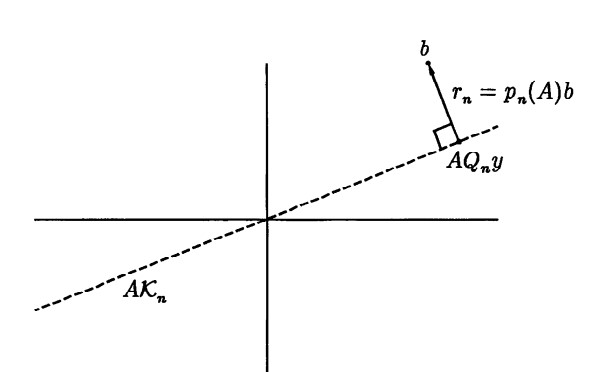
\includegraphics[scale=0.8]{GMRES-LS.jpg}
    \caption{Tìm một vector trong không gian $A \mathcal{K}_n$ \\ sao cho khoảng cách từ điểm này đến vector b nhỏ nhất}

    \label{fig:GMRES-LS}
\end{figure}

Ta xét ma trận Krylov $K_n = \begin{bmatrix} b, Ab, A^2b, \dots, A^{n-1}b \end{bmatrix}$, vì vậy:

\begin{equation}
    A K_n = \begin{bmatrix} Ab, A^2b, A^3b, \dots, A^nb \end{bmatrix}
\end{equation}

Bài toán của chúng ta là tìm một vector $c \in \mathbb{R}^n$ sao cho:

\begin{equation} \label{eq:GMRES-LS-c}
    c = \underset{c \in \mathbb{R}^{n}}{\mathrm{argmin}} \lVert b - AK_n c \rVert
\end{equation}

Với $\lVert \thickspace \rVert$ mặc định là $\lVert \thickspace \rVert_2$. Ta có thể sử dụng phân tích QR với ma trận $AK_n$. Khi đã tìm được $c$ là nghiệm của bài toán cực tiểu hóa \ref{eq:GMRES-LS-c}, $x_n=K_n c$. Nhưng bài toán trên là một bài toán không ổn định (do khi $n$ lớn ma trận $K_n$ rất gần với một ma trận kỳ dị), nên chúng ta sẽ sử dụng thuật toán lặp Arnoldi được miêu tả ở thuật toán \ref{alg:Arnoldi}
để xây dựng một dãy ma trận $Q_n$ mà các vector cột $q_1, q_2, q_3, \dots$ tạo nên cơ sở trực chuản của không gian con Krylov $\mathcal{K}_n$. Vì $x_n \in \mathcal{K}_n$, ta có thể viết $x_n = Q_n y$, bài toán cực tiểu hóa của chúng ta là tìm vector $y \in \mathbb{R}^n$, ta viết lại bài toán \ref{eq:GMRES-LS-c} dưới dạng:

\begin{equation} \label{eq:GMRES-LS-y}
    y = \underset{y \in \mathbb{R}^{n}}{\mathrm{argmin}} \lVert b - A Q_n y \rVert
\end{equation}

Ta sử dụng công thức \ref{eq:A_projection}, bài toán \ref{eq:GMRES-LS-y} có dạng:

\begin{equation}
    y = \underset{y \in \mathbb{R}^{n}}{\mathrm{argmin}} \lVert b - Q_{n+1} \widetilde{H}_n y \rVert
\end{equation}

Vì nhân một vector với một ma trận trực giao không làm thay đổi chuẩn của vector. Ta nhân các vector trong dấu $\lVert \thickspace \rVert$ với ma trận $Q_{n+1}^T$ ta được:

\begin{equation}
    y = \underset{y \in \mathbb{R}^{n}}{\mathrm{argmin}} \lVert Q_{n+1}^T b - Q_{n+1}^T Q_{n+1} \widetilde{H}_n y \rVert
\end{equation}

Trong quá trình thực hiện thuật toán lặp Arnoldi được miêu tả ở thuật toán \ref{alg:Arnoldi} để xây dựng cơ sở trực chuẩn $Q_n$ của không gian con Krylov $\mathcal{K}_n$, ta đặt $\lVert b \rVert = \beta, Q_{n+1}^T b=\lVert b \rVert e_1=\beta e_1$ với $e_1 = \begin{bmatrix}
    1 & 0 & 0 & \dots
\end{bmatrix}^T$, ta thu được dạng cuối cùng của bài toán cực tiểu hóa GMRES:

\begin{equation}
    y = \underset{y \in \mathbb{R}^{n}}{\mathrm{argmin}} \lVert \beta e_1 - \widetilde{H}_n y \rVert
\end{equation}

Tại mỗi bước $n$, ta giải bài toán cho $y$ và thu được $x_n = Q_n y$. Nhưng trong thực tế, tại mỗi bước $n$ ta không cần giải tường minh $y$ mà chỉ cần tính phần dư $\lVert \beta e_1 - \widetilde{H}_n y \rVert$, nếu phần dư này đã đủ nhỏ hơn một ngưỡng cho trước, ta sẽ dừng tại bước $n$ hiện tại và tính $x_n$. Nếu phần dư đủ nhỏ ta thực hiện bước $n+1$. Chi tiết cách tính phần dư tại mỗi bước sẽ được trình bày chi tiết ở mục sau.

Các bước cơ bản của thuật toán GMRES được trình bày ở thuật toán \ref{alg:GMRES}

Thuật toán GMRES cũng giải một bài toán xấp xỉ đa thức. Ta xét nghiệm $x_n$, tại bước $n$, vì $x_n \in \mathcal{K}_n$ nên ta có thể viết:

\begin{equation}
    x_n = c_0 b + c_1 A b + c_2 A^b + \dots + c_{n-1}A^{n-1}b=(c_0 + c_1 A + c_2 A^2 + \dots + c_{n-1} A^{n-1})b
\end{equation}

Ta đặt:

\begin{equation}
    q(z) = c_0 + c_1 z + c_2 z^2 + \dots + c_{n-1}z^{n-1}
\end{equation}

Như vậy, nghiệm tại bước thứ $n$ có thể viết dưới dạng đa thức:

\begin{equation}
    x_n = q(A)b
\end{equation}

$z(z)$ là một đa thức có bậc tối đa bằng $n-1$ với các vector hệ số $c$. Phần dư tương ứng $r_n=b - Ax_n=(I - Aq(A))b$, ta đặt đa thức $p_n(z) = 1 - z q(z)$. Như vậy ta thu được:

\begin{equation} \label{eq:Polynomial-Approximation}
    r_n = p_n(A)b
\end{equation}

Thuật toán GMRES tại mỗi bước tìm một đa thức $p_n \in P_n$ với $P_n$ là:

\begin{equation}
    P_n = \lbrace \text{là tập các đa thức có bậc } \leq n \text{ với } p(0)=1 \rbrace
\end{equation}

sao cho $p_n$ làm cực tiểu hóa phần dư (tìm vector hệ số $c$ của $p_n$):

\begin{equation} \label{eq:Find-Polynomial}
    p_n = \underset{p_n \in P_n}{\mathrm{argmin}} \lVert p_n(A)b \rVert
\end{equation}

Thuật toán GMRES cũng thỏa mãn một số tính chất bất biến như thuật toán lặp Arnoldi

\begin{dl}
    Thuật toán GMRES áp dụng cho một ma trận $A \in \mathbb{R}^{m \times m}$ thỏa mãn các tính chất sau:

    \begin{itemize}
        \item \textbf{Bất biến co dãn:} Nếu ma trận $A$ thay đổi thành $\sigma A$ với một số $\sigma \in \mathbb{R}$, và $b$ thay đổi thành $\sigma b$ thì phần dư $\lbrace r_n \rbrace$ thay đổi thành $\lbrace \sigma r_n \rbrace$.
        \item \textbf{Bất biến dưới phép biến đổi tương đương trực giao:} Nếu ma trận $A$ thay đổi thành $A A U^T$ với một ma trận $U$ trực giao bất kỳ, và $b$ thay đổi thành $Ub$, thì phần dư $\lbrace r_n \rbrace$ thay đổi thành $\lbrace U r_n \rbrace$.
    \end{itemize}
\end{dl}

Thuật toán GMRES không có tính chất bất biến tịnh tiến như thuật toán lặp Arnoldi, vì điều kiện chuẩn hóa $p(0)=1$ liên quan đến sự phụ thuộc quá trình tịnh tiến. Sự thay đổi của $\lbrace r_n \rbrace$ theo phép tịnh tiến phụ thuộc nhiều vào lựa chọn điểm gốc

\subsection{Chi tiết thực hiện thuật toán GMRES}

Một phương pháp tiêu chuẩn để giải bài toán cực tiểu hóa $y = \underset{y \in \mathbb{R}^{n}}{\mathrm{argmin}} \lVert \beta e_1 - \widetilde{H}_n y \rVert$ là phân tích ma trận $\widetilde{H}_n$ thành một một ma trận trực giao $G^T$ có kích thước $(n+1) \times (n+1)$ nhân với một ma trận tam giác trên $R$ có kích thước $(n+1) \times n$ (một ma trận mà khối $(n \times n)$ phía trên là ma trận tam giác trên và hàng cuối cùng là một vector hàng 0):

\begin{equation} \label{eq:Givens-Apply}
    \lVert r_n \rVert = \lVert G(\beta e_1 - \widetilde{H}_n y) \rVert = \lVert \beta G e_1 - R_n y \rVert
\end{equation}


Ta có thể sử dụng phương pháp phân tích Householder nhưng trong trường hợp với cấu trúc ma trận Hessenberg $\widetilde{H}_n$, ta sẽ sử dụng phương pháp ma trận quay Givens để đưa ma trận $\widetilde{H}_n$ về dạng ma trận tam giác trên.
Phương pháp ma trận quay Givens (phép quay Givens) là một phương pháp hiệu quả để tạo ra các phần tử 0 bằng cách nhân ma trận với một ma trận trực giao hạng thấp. Ví dụ: ta muốn biến đổi một ma trận $A$ thành một ma trận tam giác trên $R$ trong phân tích QR.
Ma trận Givens được ký hiệu là $G(i, k, \theta) \in \mathbb{R}^{n \times n}$ được cho bởi công thức:

\begin{equation} \label{eq:Givens-Rotation-Matrix}
    G(i, k, \theta) = \begin{bmatrix} 1 & 0 & \dots & 0 & \dots & 0 & \dots & 0 \\
                                    0 & 1 & \dots & 0 & \dots & 0 & \dots & 0 \\
                                    \vdots & \thickspace & \ddots & \thickspace & \thickspace & \thickspace & \thickspace \\
                                    0 & \thickspace & \space & c & \thickspace & s & \thickspace & 0 \\
                                    \vdots \\
                                    0 & \thickspace & \space & -s & \thickspace & c & \thickspace & 0 \\
                                    \vdots \\
                                    0 & \dots & \thickspace & \thickspace & \thickspace & \thickspace & \space & 1    \end{bmatrix}
\end{equation}

với $c = \cos(\theta), s = \sin(\theta)$. Ma trận trên tác động lên vector $x: y=G(i, k, \theta)x$

\begin{equation} \label{eq:Rotation-Result}
    y_j = \begin{cases}
        \cos(\theta) x_i + \sin(\theta) x_k, \thickspace j = i \\
        -\sin(\theta) x_i + \cos(\theta) x_k, \thickspace j = k \\
        x_j, \thickspace j \neq i, k
    \end{cases}
\end{equation}

Phép quay chọn:

\begin{equation}
    \begin{cases}
        \cos(\theta) = \dfrac{x_i}{\sqrt{x_i^2 + x_k^2}} \\
        \sin(\theta) = \dfrac{x_k}{\sqrt{x_i^2 + x_k^2}}
    \end{cases}
\end{equation}

Vì vậy $y_k = 0$. Ví dụ trong không gian hai chiều, ta quay một vector $x$ thành một vector $y$ nằm trên trục hoành. Phép quay bảo toàn độ dài của vector $x$.

Ví dụ ta xét ma trận $\widetilde{H}_4$:

\begin{equation}
    \widetilde{H}_4 = \begin{bmatrix} h_{11} & h_{12} & h_{13} & h_{14} \\
                                    h_{21} & h_{22} & h_{23} & h_{24} \\
                                    0 & h_{32} & h_{33} & h_{34} \\
                                    0 & 0 & h_{43} & h_{44} \\
                                    0 & 0 & 0 & h_{54}  \end{bmatrix}
\end{equation}

Ta áp dụng các phép quay Givens thu được:

\begin{equation}
    G(1, 2, \theta_1) \widetilde{H}_4 = \begin{bmatrix} r_{11}^{'} & r_{12}^{'} & r_{13}^{'} & r_{14}^{'} \\
        0 & r_{22}^{'} & r_{23}^{'} & r_{24}^{'} \\
        0 & h_{32} & h_{33} & h_{34} \\
        0 & 0 & h_{43} & h_{44} \\
        0 & 0 & 0 & h_{54}  \end{bmatrix}
\end{equation}

\begin{equation}
    G(2, 3, \theta_2)G(1, 2, \theta_1) \widetilde{H}_4 = \begin{bmatrix} r_{11}^{'} & r_{12}^{'} & r_{13}^{'} & r_{14}^{'} \\
        0 & r_{22}^{''} & r_{23}^{''} & r_{24}^{''} \\
        0 & 0 & r_{33}^{'} & r_{34}^{'} \\
        0 & 0 & h_{43} & h_{44} \\
        0 & 0 & 0 & h_{54}  \end{bmatrix}
\end{equation}

\begin{equation}
    G(3, 4, \theta_3)G(2, 3, \theta_2)G(1, 2, \theta_1) \widetilde{H}_4 = \begin{bmatrix} r_{11}^{'} & r_{12}^{'} & r_{13}^{'} & r_{14}^{'} \\
        0 & r_{22}^{''} & r_{23}^{''} & r_{24}^{''} \\
        0 & 0 & r_{33}^{''} & r_{34}^{''} \\
        0 & 0 & 0 & r_{44}^{'} \\
        0 & 0 & 0 & h_{54}  \end{bmatrix}
\end{equation}

\begin{equation}
    G(4, 5, \theta_4)G(3, 4, \theta_3)G(2, 3, \theta_2)G(1, 2, \theta_1) \widetilde{H}_4 = \begin{bmatrix} r_{11}^{'} & r_{12}^{'} & r_{13}^{'} & r_{14}^{'} \\
        0 & r_{22}^{''} & r_{23}^{''} & r_{24}^{''} \\
        0 & 0 & r_{33}^{''} & r_{34}^{''} \\
        0 & 0 & 0 & r_{44}^{''} \\
        0 & 0 & 0 & 0  \end{bmatrix}
\end{equation}

Tại mỗi bước $n$, chúng ta chỉ áp dụng $G(n-1, n, \theta_{n-1})G(n-2, n-1, \theta_{n-2})\dots G(1, 2, \theta_1)$ vào cột cuối cùng của ma trận $\widetilde{H}_n$, sau đó ta xác định ma trận quay $G(n, n+1, \theta_{n})$ và áp dụng vào kết quả của bước trên bởi vì $G(n, n+1, \theta_{n})$ không tác dụng lên các cột phía trước cột hiện tại (cột thứ $n$ của $\widetilde{H}_n$). Chi phí để thực hiện phân tích QR tại mỗi bước $n$ là:

\begin{itemize}
    \item Cần áp dụng $n$ ma trận quay vào cột thứ $n$ của ma trận $\widetilde{H}_n$
    \item Từ công thức \ref{eq:Rotation-Result}, mỗi bước ta cần 6 phép tính (4 phép nhân, 2 phép cộng)
\end{itemize}

Vì vậy, tại mỗi bước $n$ của thuật toán GMRES, ta cần $6n$ phép tính. Số phép tính tích lũy cần để phân tích QR cho ma trận $\widetilde{H}_n$ tính từ cột đầu tiên đến cột thứ $n=6(1+2+3+\dots+n)=6\dfrac{n(n+1)}{2}\sim \mathcal{O}(n^2)$
phép tính.

Một vấn đề nữa là chúng ta cần tìm $y$ và tính $\lVert r_n \rVert$ tại bước lặp thứ $n$.
Để tìm $y$, từ công thức \ref{eq:Givens-Apply}, ta giải $y$ bằng giải hệ phương trình lấy $n$ hàng đầu của $R_n$ và $n$ phần tử đầu của $\beta G e_1$. Đặt $\beta G e_1 = g_n$:

\begin{equation} \label{eq:GMRES-Y-Backsubstitute}
    R_n \lbrack 1:n,1:n \rbrack y = g_n \lbrack 1:n \rbrack
\end{equation}

Đây là hệ phương trình gồm $n$ phương trình và $n$ ẩn, $y$ có thể giải bằng phép thế ngược do block phía trên của $R_n$ là ma trận tam giác trên.

Để tính $\lbrack r_n \rbrack$, ta nhận thấy $r_n=g_n - R_n y$ có $n$ thành phần đầu bằng 0 do nghiệm $y$ thỏa mãn phương trình ở công thức \ref{eq:GMRES-Y-Backsubstitute}. Mặt khác do hàng cuối của $R_n$ là vector hàng 0 nên thành phần thứ $n+1$ của phần dư $r_n$ chính bằng thành phần thứ $n+1$ của $g_n$.

\begin{md}
    Chuẩn phần dư của nghiệm $x_n$ tại bước lặp thứ $n$ bằng thành phần thứ $n+1$ của vector $g_n$ thu được bằng cách nhân phía bên trái của $\beta e_1$ với liên tiếp các phép quay Givens biến đổi ma trận $\widetilde{H}_n$ thành ma trận tam giác trên.
\end{md}

Trong thực tế, khi giải các bài toán, tại mỗi bước ta thường kiểm tra chuẩn phần dư $\lVert r_n \rVert$ trước khi giải ra nghiệm $y$. Do trước khi thực hiện thuật toán, chúng ta có một ngưỡng chuẩn phần dư cho phép dừng vòng lặp $\epsilon$. Nếu tại bước hiện tại $n$, ta kiểm tra chuẩn phần dư $\lVert r_n \rvert$, nếu $\lbrack r_n \rbrack < \epsilon$ thì ta dừng vòng lặp, giải $y$ và tính $x_n=Q_n y$. Nếu không ta chuyển sang bước thứ $n+1$.

Từ các lập luận trên, ta có sơ đồ mã giả chi tiết của thuật toán GMRES được miêu tả ở thuật toán \ref{alg:GMRES-Detailed}:

\begin{algorithm}
    \caption{Các bước chi tiết thuật toán GMRES}\label{alg:GMRES-Detailed}
    \begin{algorithmic}
        \State{Cho ma trận $A$ không kỳ dị, $b$, chuẩn phần dư $\epsilon$ cho phép}
        \State{$q_1 \leftarrow b/\lVert b \rVert$}
        \State{$\beta \leftarrow \lVert b \rVert$}
        \State{$g_0 \leftarrow \beta e_1$}
        \For {$n=1,2,3,\dots$}
            \State {Thực hiện bước thứ n của thuật toán \ref{alg:Arnoldi} thu được $q_{n+1}$ và cột thứ $n$ của ma trận $\widetilde{H}_n$}
            \State {Tính $G(n-1, n, \theta_{n-1})G(n-2, n-1, \theta_{n-2})\dots G(1, 2, \theta_1)$ vào cột cuối cùng của ma trận $\widetilde{H}_n$}
            \State {Tính ma trận quay $G(n, n+1, \theta_n)$ từ kết quả của bước trên và áp dụng vào kết quả này}
            \State {$g_{n-1} \leftarrow \begin{bmatrix} g_{n-1} & 0 \end{bmatrix}$}
            \State {$g_n \leftarrow G(n, n+1, \theta_n) g_{n-1}$}
            \If {Nếu thành phần thứ $n+1$ của $g_n < \epsilon$ }
                \State {Giải $y$ từ phương trình $R_n \lbrack 1:n,1:n \rbrack y = g_n \lbrack 1:n \rbrack$}
                \State {$x_n \leftarrow Q_n y$}
                \State {break}
            \EndIf
        \EndFor
    \end{algorithmic}
\end{algorithm}

\subsection{Một số đặc điểm của thuật toán GMRES} \label{GMRES-Characteristic}


\subsubsection{Chi phí bộ nhớ}

Thuật toán GMRES yêu cầu một lượng lớn bộ nhớ và trở nên rất đắt khi số bước lặp cao.
Yêu cầu về bộ nhớ cơ bản là lưu các vector $b, x \in \mathbb{R}^{m}$ và ma trận $A \in \mathbb{R}^{m \times m}$. Nếu $A$ là ma trận thưa, mỗi hàng có $l$ phần tử khác 0 thì yêu cầu về bộ nhớ cần lưu $(l+2)m$ số thực để tạo bài toán. Thuật toán GMRES cần phải lưu tất cả các vector $q_1, q_2, \dots, q_n$. Từng vector $q_i \in \mathbb{R}^{m}, i=1\dots n$, vì vậy cần chi phí bộ nhớ là $mn$ số thực.
Ngoài ra ta cần giải bài toán cực tiểu hóa, ta thu được $y \in \mathbb{R}^n$, tại bước lặp thứ $n$ $x_n = Q_n y$ (nếu thỏa mãn điều kiện hội tụ là $\lVert r_n \rVert < \epsilon$), ta cần lưu $n$ số thực cho $y$.
Chúng ta cũng cần lưu ma trận $\widetilde{H}_n$, thực tế chúng ta lưu ma trận $R_n \in \mathbb{R}^{n \times n}$ với chi phí $\dfrac{n^2 + n}{2}$.
Cuối cùng chúng ta cần lưu các ma trận quay Givens, mỗi ma trận quay cần lưu hai số $\sin$ và $\cos$. Tại bước thứ $n$, cần lưu $n$ ma trận quay Givens từ $\sin(\theta_1),\dots, \sin(\theta_n)$ và $\cos(\theta_1),\dots,\cos(\theta_n)$ như vậy chi phí là $2n$.
Tổng hợp lại chi phí bộ nhớ cho thuật toán GMRES tại bước thứ $n$ là: $(l+2)m + mn + n + \dfrac{n^2 + n}{2} + 2n$.

\subsubsection{Chi phí tính toán}

Tại mỗi bước $n$, của thuật toán GMRES, ta cần thực hiện các công việc:

\begin{itemize}
    \item Thực hiện thuật toán Arnoldi để thu được vector $q_{n+1}$ và cột thứ $n$ của ma trận $\widetilde{H}_n$. Bước này chi phí là: \begin{itemize}
        \item Tính $Aq_n$ cần $m(2m-1)$ phép tính
        \item $n$ bước, mỗi bước gồm 1 phép nhân vô hướng ($h_{j,n} \leftarrow q_j^Tv$) cần $2m-1$ phép tính và một bước nhân 1 số ($h_{j,n}q_j$) với một vector cần $m$ phép tính và một bước trừ hai vector cần $m$ phép tính ($v \leftarrow v - h_{j,n}q_j$). Như vậy bước này cần $n(4m-1)$ phép tính.
        \item Một bước tính chuẩn ($h_{n+1,n} \leftarrow \lVert v \rVert$) cần $2m-1$ phép tính.
        \item Một bước chuẩn hóa ($q_{n+1} \leftarrow v/h_{n+1,n}$) cần $m$ phép tính.
    \end{itemize}
    Như vậy số phép tính để thực hiện thuật toán Arnoldi cần $m(2m-1) + n(4m-1) + 2m-1 + m=m(2m-1) + n(4m-1)+ 3m-1=2m^2+4mn+2m-n-1$.
    \item Bước áp dụng phép quay Givens cho cột thứ $n$ của ma trận $\widetilde{H}_n$ gồm $6n+10$ ($10$ là số phép tính để tính $\sin(\theta_n)$ và $\cos(\theta_n)$).
    \item Bước cập nhật $g_n \leftarrow G(n, n+1, \theta_n)g_{n-1}$ cần 6 phép tính
\end{itemize}

Như vậy tại bước thứ $n$ của thuật toán GMRES ta cần số phép tính là: $2m^2+4mn+2m-n-1 + 6n+10 + 6=2m^2+4mn+2m+5n+15$ phép tính.

Nếu giả sử tại bước $n$, điều kiện hội tụ đã thỏa mãn $\lVert r_n \rVert < \epsilon$, ta cần thêm bước giải $y$ bằng phép thế ngược. Để giải hệ ở phương trình \ref{eq:GMRES-Y-Backsubstitute}, tại bước thế ngược thứ $k, k=1,2,\dots,n$, ta cần số phép tính:
\begin{itemize}
    \item 1 phép chia
    \item $k-1$ phép nhân
    \item $k-1$ phép trừ
\end{itemize}

Vậy số bước cần để giải hệ phương trình \ref{eq:GMRES-Y-Backsubstitute} là $n + 2\lbrack 0 + 1 + \dots + (k-1) + \dots + (n-1)\rbrack=n+(n-1)n=n^2$ phép tính

Ngoài ra ta cần tính $x_n = Q_n y$ cần $m(2n-1)$ phép tính

Ta tổng hợp số phép tính tích lũy từ khi bắt đầu đến khi nhận được lời giải sử dụng thuật toán GMRES là: $2m^2 n + 4m\dfrac{n(n+1)}{2}+2mn + 5\dfrac{n(n+1)}{2}+15n+n^2+m(2n-1)=2m^2 n + 2mn^2+4mn+3.5n^2+3m+15n+2.5 \sim \mathcal{O}(2m^2n+ 2mn^2)$

Ta thấy chi phí tính toán là một nhược điểm lớn của GMRES, do tại mỗi bước $n$, chi phí tính toán phần thực hiện thuật toán lặp Arnoldi phụ thuộc vào $n$ ($2m^2+4mn+2m+5n+15$) khiến cho $n$ càng lớn thì chi phí tính toán càng lớn, bước sau chi phí tính toán nhiều hơn bước trước. Đây là vấn đề cần được cải thiện đối với thuật toán GMRES.

\subsubsection{Sự hội tụ của thuật toán GMRES} \label{GMRES-Convergence}

Ta nhận thấy có hai quan sát với phần dư của thuật toán GMRES:

\begin{itemize}
    \item $ \lVert r_{n+1} \rVert \leq \lVert r_{n} \rVert $. Lý do là vì $\lVert r_n \rVert$ nhỏ nhất có thể trong không gian con Krylov thứ $n$ $\mathcal{K}_n$, khi mở rộng không gian con Krylov $\mathcal{K}_n$ sang $\mathcal{K}_{n+1}$, chuẩn phần dư chỉ có thể giảm hoặc tệ nhất là chuẩn phần dư không thay đổi.
    \item Mặt khác sau khi thực hiện $m$ bước lặp, quá trình phải hội tụ hay $\lVert r_m \rVert=0$. $\lVert r_m \rVert = 0$ sẽ xảy ra khi $\mathcal{K}_m = \mathbb{R}^m$ và trong trường hợp đặc biệt nếu vector $b \in \mathcal{K}_n$ với một số $n < m$, thì sự hội tụ sẽ xảy ra sớm hơn. $\lVert r_m \rVert = 0$ chỉ có ý nghĩa về mặt lý thuyết của thuật toán GMRES nhưng không có nhiều ý nghĩa về mặt thực tiễn, chúng ta mong rằng GMRES sẽ hội tụ sau $n$ bước nhỏ hơn rất nhiều so với $m$.
\end{itemize}

Để thu được nhiều thông tin hữu ích hơn về quá trình hội tụ của thuật toán GMRES, ta phải sử dụng bài toán xấp xỉ đa thức đã được đề cập ở mục \ref{GMRES-Introduction}. Từ công thức \ref{eq:Polynomial-Approximation}, ta biết rằng: $\lVert r_n \rVert=\lVert p_n(A)b \rVert \leq \lVert p_n(A) \rVert \lVert b \rVert$. Ngoại trừ trường hợp $b$ có cấu trúc đặc biệt liên quan đến ma trận $A$ thì nhân tố quan trọng xác định $ \lVert r_n \rVert$ là $\lVert p_n(A) \rVert$. Bất đẳng thức xác định tốc độ hội tụ của thuật toán GMRES là:

\begin{equation} \label{eq:GMRES-Convergence-Rate}
    \dfrac{\lVert r_n \rVert}{\lVert b \rVert} \leq \inf_{p_n \in P_n} \lVert p_n(A) \rVert
\end{equation}

Ta cần phân tích với một ma trận $A$ và một số $n$ cho trước thì $\lVert p_n(A) \rVert$ có thể nhỏ bao nhiêu. Cách tiếp cận tiêu chuẩn là tìm một đa thức $p(z)$ sao cho $p(z)$ càng nhỏ càng tốt trên tập phổ của ma trận $A$ $\Lambda(A)$ và thỏa mãn $p(0)=1$. Ta giả sử ma trận $A$ là ma trận chéo hóa được, thỏa mãn $A=V\Lambda V^{-1}$ với $V$ là ma trận không kỳ dị và $\Lambda$ là ma trận đường chéo. Ta có bất đẳng thức:

\begin{equation}
    \lVert p_n(A) \rVert \leq \lVert V \rVert \lVert p_n(\Lambda) \rVert \lVert V^{-1} \rVert = \dfrac{\max(\sigma(V))}{\min(\sigma(V))} \lVert p_n(\Lambda) \rVert = \kappa(V) \lVert p_n(\Lambda) \rVert
\end{equation}

Từ công thức trên và công thức \ref{eq:GMRES-Convergence-Rate}, ta đi đến định lý:

\begin{dl} \label{dl:GMRES-Convergence-Rate}
    Tại bước thứ $n$ của thuật toán GMRES, phần dư $r_n$ thỏa mãn:
    \begin{equation}
        \dfrac{\lVert r_n \rVert}{\lVert b \rVert} \leq \inf_{p_n \in P_n} \lVert p_n(A) \rVert \leq \kappa(V) \inf_{p_n \in P_n} \lVert p_n \rVert_{\Lambda(A)}
    \end{equation}
    với $\Lambda(A)$ là tập các giá trị riêng của ma trận $A$, $V$ là ma trận không kỳ dị của các vector riêng của ma trận $A$ (giả sử ma trận $A$ chéo hóa được), và $\lVert p_n \rVert_{\Lambda(A)}=\underset{z \in \Lambda(A)}{\sup} \lvert p_n(z) \rvert$
\end{dl}

Ý nghĩa của định lý \ref{dl:GMRES-Convergence-Rate} là nếu ma trận $A$ có số điều kiện của ma trận $V$ là $\kappa(V)$ không quá lớn và một đa thức thuộc tập $P_n$ được tìm thấy mà độ lớn của nó trên phổ của ma trận $A$ là $\Lambda(A)$ giảm nhanh theo $n$ thì thuật toán GMRES hội tụ nhanh.

Thuật toán GMRES sẽ hội tụ khi ta thực hiện số bước lặp bằng với số giá trị riêng riêng biệt của ma trận $A$. Sự hội tụ sẽ phụ thuộc vào cấu trúc các giá trị riêng của ma trận $A$ được phân bố thế nào.
Từ bài toán tìm đa thức $p_n \in P_n$ được nêu ở công thức \ref{eq:Find-Polynomial}, ta đặt đa thức $p_n$ có dạng:

\begin{equation}
    p_n(z) = 1 - \sum_{i=1}^n c_i z^i
\end{equation}

Trong quá trình giải bài toán cực tiểu bằng việc tìm đa thức mà giá trị của nó nhỏ trên phổ của ma trận $A$ hay giá trị của nó nhỏ với mọi giá trị riêng của ma trận $A$. Trong trường hợp đặc biệt nếu $n$ lớn hơn số giá trị riêng của ma trận $A$ thì đa thức này sẽ bằng 0 tại mọi giá trị riêng của ma trận $A$ và thuộc $P_n$.
Nhưng đôi khi chúng ta chỉ hy vọng tìm được một đa thức mà có giá trị đủ nhỏ tại tất cả các giá trị riêng. Việc tìm đa thức sẽ càng dễ hơn nếu các giá trị riêng phân thành các nhóm mà mỗi nhóm các giá trị riêng nằm sát nhau và khó hơn nếu các giá trị riêng có các giá trị riêng biệt và nằm ra nhau. Và việc phân bố các giá trị riêng của ma trận $A$ có mối quan hệ mật thiết với số điều kiện của ma trận $A$.

Nếu $\kappa(V)$ nhỏ thì ta có hai trường hợp:
\begin{itemize}
    \item Nếu ma trận $A$ đối xứng xác định dương thì thuật toán GMRES cần $O(\sqrt{\kappa})$ bước để hội tụ.
    \item Nếu ma trận $A$ không xác định dấu thì thuật toán GMRES cần $O(\kappa)$ bước để hội tụ.
\end{itemize}

Nếu ma trận $A$ là một ma trận không chéo hóa được, nếu $n^{*}$ là số chiều của \textit{không gian bất biến tổng quát nhỏ nhất} chứ vector $b$, thuật toán GMRES sẽ dừng sau đúng $n^{*}$ bước. Một không gian $\mathcal{S}$ được gọi là \textit{không gian con bất biến tổng quát} nếu $v \in \mathcal{S} \Rightarrow A^{n}v \in \mathcal{S} \thickspace \forall n \geq 0$ 

Nếu ma trận $A=VJV^{-1}$ với ma trận $J$ là một ma trận có dạng chuẩn Jordan thì:

\begin{equation}
    \lVert p_n(A) \rVert \leq \lVert V \rVert \lVert p_n(J) \rVert \lVert V^{-1} \rVert=\dfrac{\max(\sigma(V))}{\min(\sigma(V))} \lVert p_n(J) \rVert = \kappa(V) \lVert p_n(J) \rVert
\end{equation}

và:

\begin{equation}
    \dfrac{\lVert r_n \rVert}{\lVert b \rVert} \leq \inf_{p_n \in P_n} \lVert p_n(A) \rVert \leq \kappa(V) \inf_{p_n \in P_n} \lVert p_n(J) \rVert
\end{equation}

Để đánh giá $\inf_{p_n \in P_n} \lVert p_n(J) \rVert$ khá phức tạp, giá trị này được phân tích rất kỹ trong \cite{tichy2005worst}.


\subsection{Cải thiện thuật toán GMRES}

\subsubsection{Phương pháp khởi tạo lại}

Từ các phân tích ở mục \ref{GMRES-Characteristic}, ta thấy rằng chi phí về lưu trữ bộ nhớ và chi phí tính toán tăng theo $n$. Đây là nhược điểm rất lớn của thuật toán GMRES, vì vậy trong thực tế ta sẽ hay sử dụng phương pháp khởi tạo lại.
Ý tưởng của phương pháp này là chọn giới hạn số bước lặp $n_{\max}$. Khi $n$ đạt đến $n_{\max}$ mà thuật toán GMRES chưa hội tụ, ta tính $x_{n_{\max}}$ và bỏ tất cả các vector trực giao $q_1, q_2, \dots, q_{n_{\max}}$ chỉ giữ lại nghiệm tại bước lặp $x_{n_{\max}}$. Đặt $x_{n_{\max}}=x_0$, ta quay trở lại giải hệ phương trình:

\begin{equation} \label{eq:Restart-Equation}
    A(x - x_0) = b - A x_0 = r_0
\end{equation}

Cách giải hệ phương trình \ref{eq:Restart-Equation} hoàn toàn tương tự như trình tự đã được trình bày ở thuật toán \ref{alg:GMRES-Detailed} chỉ khác là vai trò của $b$ đã được thay bằng $r_0$ và $x_n$ được thay bằng $x_0+Q_n y$

\begin{algorithm}
    \caption{Các bước chi tiết thuật toán GMRES khởi tạo lại}\label{alg:GMRES-Restart}
    \begin{algorithmic}
        \State{Cho ma trận $A$ không kỳ dị, $b$, $n_{\max}$, chuẩn phần dư $\epsilon$ cho phép}
        \State{$x_0 \leftarrow 0$}
        \State{$r_0 \leftarrow b - A x_0$}
        \State{$q_1 \leftarrow r_0 / \lVert r_0 \rVert$}
        \State{$\beta \leftarrow \lVert r_0 \rVert$}
        \State{$g_0 \leftarrow \beta e_1$}
        \For {$n=1,2,3,\dots, n_{\max}$}
            \State {Thực hiện bước thứ n của thuật toán \ref{alg:Arnoldi} thu được $q_{n+1}$ và cột thứ $n$ của ma trận $\widetilde{H}_n$}
            \State {Tính $G(n-1, n, \theta_{n-1})G(n-2, n-1, \theta_{n-2})\dots G(1, 2, \theta_1)$ vào cột cuối cùng của ma trận $\widetilde{H}_n$}
            \State {Tính ma trận quay $G(n, n+1, \theta_n)$ từ kết quả của bước trên và áp dụng vào kết quả này}
            \State {$g_{n-1} \leftarrow \begin{bmatrix} g_{n-1} & 0 \end{bmatrix}$}
            \State {$g_n \leftarrow G(n, n+1, \theta_n) g_{n-1}$}
            \If {Nếu thành phần thứ $n+1$ của $g_n < \epsilon$ }
                \State {Giải $y$ từ phương trình $R_n \lbrack 1:n,1:n \rbrack y = g_n \lbrack 1:n \rbrack$}
                \State {$x_n \leftarrow x_0 + Q_n y$}
                \State {break}
            \EndIf

            \If {$n = n_{\max}$}
                \State {Giải $y$ từ phương trình $R_{n_{\max}} \lbrack 1:n_{\max},1:n_{\max} \rbrack y = g_{n_{\max}} \lbrack 1:n_{\max} \rbrack$}
                \State {$x_{n_{\max}} \leftarrow x_0 + Q_{n_{\max}} y$}
                \State {$x_0 \leftarrow x_{n_{\max}}$}
                \State{$r_0 \leftarrow b - A x_0$}
                \State{Xóa $Q_{n_{\max}}$}
                \State{$q_1 \leftarrow r_0 / \lVert r_0 \rVert$}
                \State{$\beta \leftarrow \lVert r_0 \rVert$}
                \State{$g_0 \leftarrow \beta e_1$}
                \State{Quay trở lại vòng lặp for ban đầu}
            \EndIf
        \EndFor
    \end{algorithmic}
\end{algorithm}

Phương pháp khởi tạo lại có ưu điểm là khiến cho chi phí bộ nhớ và chi phí tính toán tại mỗi bước là không quá lớn. Đặc biệt việc giới hạn không cho phép lượng bộ nhớ quá lớn phải sử dụng, nếu không giới hạn số bước thì rất có thể bộ nhớ trong hệ thống thực thi thuật toán GMRES dễ bị tràn.

Nhược điểm của phương pháp là khiến cho thuật toán GMRES lâu hội tụ hơn. Nếu $n_{\max}$ quá lớn vẫn có thể khiến cho bộ nhớ bị tràn hoặc chi phí tính toán trong từng bước lớn. Nếu $n_{\max}$ nhỏ có thể khiến thuật toán GMRES gần như không bao giờ hội tụ. Việc chọn $n_{\max}$ tối ưu vẫn là một câu hỏi mở.

\subsubsection{Phương pháp điều kiện đầu}

Thay vì giới hạn số bước lặp cho phép của thuật toán GMRES, đôi khi người ta sẽ cải thiện sự hội tụ của thuật toán bằng cách thay đổi cấu trúc giá trị riêng của ma trận $A$ từ đó làm giảm số bước lặp cần thiết để thuật toán hội tụ.
Từ những phân tích ở tiểu mục \ref{GMRES-Convergence}, ta nhận thấy thuật toán GMRES hội tụ rất nhanh nếu ma trận $A$ có một số ít các giá trị riêng riêng biệt hoặc các giá trị riêng tập trung thành số ít các cụm. Vì vậy một ý tưởng tự nhiên là biến đổi ma trận $A$ bằng cách nhân ma trận $A$ với một ma trận $M$ (có thể nhân $M$ vào bên trái hoặc bên phải ma trận $A$ hoặc từ hai phía) mà kết quả là một ma trận có những đặc tính mong muốn giúp cho thuật toán hội tụ nhanh.
Ta xét hệ phương trình $Ax=b$. Một ma trận điều kiện đầu $M$ thay đổi hệ phương trình thành:

\begin{equation}
    M^{-1}Ax = M^{-1}b
\end{equation}

được gọi là điều kiện đầu bên trái. Hay:

\begin{equation}
    AM^{-1}y = b
\end{equation}

được gọi là điều kiện đầu bên phải với $x=M^{-1}y$. Hay:

\begin{equation}
    L^{-1}AU^{-1}z = L^{-1}b
\end{equation}

được gọi là điều kiện đầu phân tách với $x=U^{-1}z$

Điều kiện để chọn được một ma trận điều kiện đầu tốt cần thỏa mãn những yêu cầu (giả sử điều kiện đầu đang xét là điều kiện đầu bên trái):

\begin{itemize}
    \item $\kappa(M^{-1}A)\approx 1$
    \item Phổ của ma trận $M^{-1}A$ gồm ít các ma trận riêng biệt hoặc các giá trị riêng tập trung theo số ít cụm.
    \item Ma trận $M$ có thể được xây dựng bởi chi phí tính toán đủ thấp.
\end{itemize}

\section{Thuật toán MINRES}

\subsection{Giới thiệu thuật toán MINRES}

Chương trước đã trình bày về thuật toán GMRES. Mặc dù thuật toán MINRES là đối tượng chính được đề cập trong tiểu luận nhưng thuật toán GMRES được trình bày rất chi tiết, mục đích là để có thể dễ dàng so sánh sự giống nhau và khác nhau của hai thuật toán trên nhiều khía cạnh. Thuật toán MINRES áp dụng cho bài toán giải hệ phương trình $Ax=b$ với ma trận $A \in \mathbb{R}^{m \times m}$ là ma trận đối xứng không xác định dấu và có thể là ma trận kỳ dị, vector $b \in \mathbb{R}^m$, ma trận $A \neq 0$ và vector $b \neq 0$

Thuật toán MINRES có nhiều điểm tương đồng với thuật toán GMRES. Thuật toán MINRES có thể xem như là thuật toán GMRES áp dụng cho ma trận đối xứng không xác định dấu.
Thuật toán lặp Arnoldi trở thành thuật toán lặp Lanczos hay còn gọi là phương pháp truy hồi ba tham số.

Ta cần kiểm chứng hệ vector được tạo thành từ thuật toán lặp Lanczos cũng là hệ cơ sở trực chuẩn giống như thuật toán lặp Arnoldi khi ma trận $A$ là ma trận đối xứng. Đặt $\tilde{q}_{n+1}=Aq_{n} - \alpha_n q_n - \beta_{n-1}q_{n-1}$
Ta xét tích vô hướng $\tilde{q}_{n+1}^T q_{n-1}$:

\begin{equation}
    \begin{aligned}
        \tilde{q}_{n+1}^T q_{n-1}&=(Aq_{n} - \alpha_n q_n - \beta_{n-1}q_{n-1})^T q_{n-1} \\
        & = (Aq_{n})^T q_{n-1} - \beta_{n-1}\\
        & =q_{n}^T (Aq_{n-1}) - \beta_{n-1}=q_n^T(\tilde{q}_n^T + \alpha_{n-1}q_{n-1} + \beta_{n-2}q_{n-2})-\beta_{n-1} \\
        &= \beta_{n-1} - \beta_{n-1} = 0
    \end{aligned}
\end{equation}

Với $k < n-1$, ta xét tích vô hướng $\tilde{q}_{n+1}^T q_k$:

\begin{equation}
    \begin{aligned}
        \tilde{q}_{n+1}^T q_k &= (A q_n - \alpha_n q_n - \beta_{n-1} q_{n-1})^T q_k \\
        &= (Aq_n)^T q_k \\
        &= q_n^T (Aq_k)=q_n^T (\tilde{q}_k + \alpha_k q_k + \beta_{k-1} q_{k-1})=0
    \end{aligned}
\end{equation}

Vì vậy, các vector $q_1, q_2, \dots, q_{n+1}$ tạo thành một hệ cơ sở trực chuẩn của không gian con Krylov.

Giống như thuật toán GMRES, tại mỗi bước $n$, ta tìm một điểm $x_n$ sao cho cực tiểu hóa phần dư $r_n=b - Ax_n$
Ta xét lại công thức \ref{eq:AQHQ}, vì $A = A^T$ nên ta có:

\begin{equation}
    A = QHQ^T = A^T = QH^TQ^T \Rightarrow H = H^T
\end{equation}

Vì vậy ma trận $H$ trong trường hợp ma trận $A$ đối xứng có dạng 3 đường chéo $T$
Vì $x_n \in \mathcal{K}_n$, ta có thể viết $x_n = Q_n y$ với $y \in \mathbb{R}^n$ là tọa độ của $x_n$ trong $\mathcal{K}_n$. Ta tìm vector $y \in \mathbb{R}^n$ cực tiểu hóa hàm mục tiêu:

\begin{equation} \label{eq:MINRES-Least-Square-Problem}
    y = \underset{y \in \mathbb{R}^n}{\mathrm{argmin}} \lVert b - AQ_n y \rVert
\end{equation}

Ta sử dụng công thức \ref{eq:Three-term-recurrence}, bài toán cực tiểu hóa \ref{eq:MINRES-Least-Square-Problem} có dạng:

\begin{equation}
    y = \underset{y \in \mathbb{R}^n}{\mathrm{argmin}} \lVert b - Q_{n+1} \widetilde{T}_{n+1} y \rVert
\end{equation}

Ở trong dấu $\lVert \thickspace \rVert$ của công thức trên ta nhân bên trái với ma trận trực giao $Q_{n+1}^T$ ta được:

\begin{equation}
    y = \underset{y \in \mathbb{R}^n}{\mathrm{argmin}} \lVert Q_{n+1}^T(b - Q_{n+1} \widetilde{T}_{n+1} y) \rVert
\end{equation}

Cũng như thuật toán GMRES, ta đặt $\lVert b \rVert= \beta, Q_{n+1}^T b=\beta e_1$, dạng cuối cùng của bài toán cực tiểu hóa MINRES:

\begin{equation}
    y = \underset{y \in \mathbb{R}^n}{\mathrm{argmin}} \lVert \beta e_1 - \widetilde{T}_{n+1} y \rVert 
\end{equation}



\begin{algorithm}
    \caption{Thuật toán MINRES}\label{alg:MINRES}
    \begin{algorithmic}
        \State{Gán $q_1 \leftarrow b/\lVert b \rVert$}
        \For {$n=1,2,3,\dots$}
            \State {Thực hiện bước thứ n của thuật toán \ref{alg:Lanczos}}
            \State {Tìm $y$ để cực tiểu hóa $\lVert \beta e_1 - \widetilde{T}_n y \rVert_2=\lVert r_n \rVert_2$}
            \State {$x_n \leftarrow Q_n y$}
        \EndFor
    \end{algorithmic}
\end{algorithm}

Tại mỗi bước $n$, ta có thể thu được $x_n$ bằng cách tương tự như GMRES là giải bài toán cho $y$ và thu được $x_n = Q_n y$ hoặc một cách thuận tiện và tiết kiệm bộ nhớ hơn ta thu được $x_n$ từ $x_{n-1}$ mà không cần lưu các vector $q_1, q_2, \dots, q_n$. Ưu điểm dễ thấy nhất của cách thứ hai là ta không cần tốn chi phí bộ nhớ cho ma trận $Q_n$.
Cách tính chuẩn phần dư cũng tương tự như thuật toán GMRES. Chi tiết thực hiện thuật toán GMRES sẽ được trình bày ở mục sau.

Các bước cơ bản của thuật toán MINRES được trình bày ở thuật toán \ref{alg:MINRES}

Do thuật toán MINRES là trường hợp đặc biệt của thuật toán GMRES nên MINRES cũng giải một bài toán xấp xỉ đa thức. Hay nói cách khác là tìm một đa thức $p_n \in P_n$ làm cực tiểu hóa phần dư $r_n = p_n(A)b$:
\begin{equation}
    p_n = \underset{p_n \in P_n}{\mathrm{argmin}} \lVert p_n(A)b \rVert
\end{equation}

\subsection{Chi tiết thực hiện thuật toán MINRES}

Phương pháp để giải bài toán $y=\underset{y \in \mathbb{R}^n}{\mathrm{argmin}} \lVert \beta e_1  \rVert$ là phân tích ma trận $\widetilde{T}_n$ thành một ma trận trực giao $G^T$ có kích thước $(n+1) \times (n+1)$ nhân với một tam giác trên $R$ có kích thước $(n+1) \times n$:

\begin{equation}
    \lVert r_n \rVert = \lVert G(\beta e_1 - \widetilde{T}_n y) \rVert = \lVert \beta G e_1 - R_n y \rVert
\end{equation}

Ta xem lại cấu trúc của ma trận ba đường chéo $\widetilde{T_n}$:

\begin{equation}
    \widetilde{T}_n = \begin{bmatrix}
        \alpha_1 & \beta_1 & \space & \space & \space \\
        \beta_1 & \alpha_2 & \beta_1 & \space & \space \\
        \space & \beta_2 & \alpha_3 & \ddots & \space \\
        \space & \space & \ddots & \ddots & \beta_{k-1} \\
        \space & \space & \space & \beta_{k-1} & \alpha_k \\
        \space & \space & \space & \space & \beta_{n}
    \end{bmatrix}
\end{equation}

Ta vẫn sử dụng phương pháp ma trận quay Givens nhưng trong trường hợp ma trận $\widetilde{T}_n$, cấu trúc của ma trận $\widetilde{T}_n$ tạo ra một vài khác biệt trong quá trình tính toán:

\begin{itemize}
    \item Mỗi ma trận quay $G(n, n+1, \theta_n)$ chỉ thực sự có hiệu lực trên ba cột $n, n+1, n+2$ của ma trận $\widetilde{T}_n$.
    \item Mỗi cột thứ $n$ chỉ áp dụng ba ma trận quay $G(n-2, n-1, \theta_{n-2}), G(n-1, n, \theta_{n-1})$ (được tính ở các hai bước liền kề $n-2$ và $n-1$) và $G(n, n+1, \theta_n)$. Ngoại trừ hai cột đầu tiên của ma trận $\widetilde{T}_n$, cột đầu tiên chỉ được áp dụng duy nhất ma trận $G(1, 2, \theta_1)$ và cột thứ hai được áp dụng hai ma trận $G(1, 2, \theta_1), G(2, 3,\theta_2)$.
\end{itemize}

với các ma trận quay Givens được định nghĩa trong công thức \ref{eq:Givens-Rotation-Matrix}.

Như vậy, sau khi thực hiện phân tích QR cho ma trận $\widetilde{T}_n$ ta thu được ma trận $R_n$ là ma trận tam giác trên nhưng chỉ có ba đường chéo liền kề nhau:

\begin{equation}
    R_n = \begin{bmatrix}
        \gamma_1 & \delta_2 & \epsilon_3 & \space & \space & \space & \space \\
        \space & \gamma_2 & \delta_3 & \epsilon_4 & \space & \space & \space \\
        \space & \space  & \gamma_3 & \delta_4 & \epsilon_5 & \space & \space \\
        \space & \space & \space & \ddots & \ddots & \ddots & \space \\
        \space & \space & \space & \space & \gamma_{k-2} & \delta_{k-1} & \epsilon_k \\
        \space & \space & \space & \space & \space & \gamma_{k-1} & \delta_k \\
        \space & \space & \space & \space & \space & \space & \gamma_k
    \end{bmatrix}
\end{equation}

\section{So sánh phương pháp GMRES và phương pháp MINRES}

Phương pháp GMRES và MINRES là các phương pháp lặp trên không gian con Krylov để giải hệ phương trình $Ax=b$ trong các trường hợp tổng quan hơn phương pháp Gradient liên hợp.
MINRES được sử dụng để giải các hệ phương trình mà ma trận $A$ là ma trận đối xứng, còn phương pháp GMRES để giải các hệ phương trình mà ma trận $A$ là ma trận không kỳ dị.
Hai phương pháp này gần giống với phương pháp Gradient liên hợp nhưng phương pháp Gradient liên hợp cực tiểu hóa hàm mục tiêu $\displaystyle \min_{x \in \mathcal{K}_n}\dfrac{1}{2}x^TAx - x^Tb$,
trong khi hai phương pháp GMRES và MINRES tìm vector trong không gian con Krylov thứ n $\displaystyle \mathcal{K}_n$ mà làm cực tiểu hóa phần dư $\displaystyle \min_{x \in \mathcal{K}_n}\dfrac{1}{2}\lVert b - Ax \rVert_2^2$

Hai phương pháp GMRES và MINRES giải các bài toán tối ưu hóa có ràng buộc, nói chung là bài toán khá khó giải. Xét $x_n \in \mathcal{K}_n$, ta có thể biểu diễn $x_n$ dạng:
$x_n = Q_n y$ với $y$ là tọa độ của $x_n$ trong hệ cơ sở trực chuẩn của không gian Krylov thứ n $\mathcal{K}_n$. Hàm mục tiêu trở thành:
\begin{equation} \min_{y \in \mathbb{R}^{n}}  \lVert b - AQ_n y \rVert_2^2\end{equation}

Như vậy bài toán đã được đưa về bài toán tối ưu có ràng buộc với số chiều của $y$ nhỏ hơn so với $x$. Tuy nhiên với ma trận $A$ có kích thước lớn thì bài toán trên vẫn khá đắt.

Nhưng chúng ta có thể giảm số chiều của bài toán đi nữa bằng cách nhân hàm mục tiêu với ma trận trực giao $Q_{n+1}$ là ma trận cơ sở trực chuẩn của không gian con Krylov thứ n+1:
\begin{equation} \min_{y \in \mathbb{R}^{n}}  \lVert b - AQ_n y \rVert_2^2 = \min_{y \in \mathbb{R}^{n}}  \lVert Q_{n+1}^T(b - AQ_n y) \rVert_2^2 \label{eq:uncons_obj}\end{equation}

Ta sử dụng công thức:

\begin{equation}
    AQ_n = Q_{n+1}\widetilde{H}_n
\end{equation}

đối với phương pháp GMRES, đối với phương pháp MINRES:
\begin{equation}
    AQ_n = Q_{n+1} \widetilde{T}_n
\end{equation}
trong đó, $\widetilde{H}_n$ là ma trận Hessenberg có dạng ở công thức \ref{eq:Hessenberg_matrix}:
và ma trận $\widetilde{T}_n$ là ma trận 3 đường chéo được đề cập ở công thức \ref{eq:Trigonal_Matrix}:

Với $\lVert b \rVert = \beta, q_1 = \dfrac{b}{\beta}$, hàm mục tiêu \eqref{eq:uncons_obj} trở thành:

\begin{equation}
    \min_{y \in \mathbb{R}^{n}}  \lVert Q_{n+1}^T(b - AQ_n y) \rVert_2^2=\min_{y \in \mathbb{R}^{n}} \lVert \beta e_1 - \widetilde{H}_n y\rVert_2^2
\end{equation}

đối với phương pháp GMRES (ma trận A là ma trận không suy biến).
Đối với phương pháp MINRES (ma trận A là ma trận đối xứng):
\begin{equation}
    \min_{y \in \mathbb{R}^{n}}  \lVert Q_{n+1}^T(b - AQ_n y) \rVert_2^2=\min_{y \in \mathbb{R}^{n}} \lVert \beta e_1 - \widetilde{T}_n y\rVert_2^2
\end{equation}

Như vậy, bài toán được đưa về một bài toán bình phương tối thiểu với kích thước $(n+1)\times n$

\begin{equation}
    y_n = \operatorname*{argmin}_{y_n \in \mathbb{R}^{n}} \lVert \beta e_1 - \widetilde{H}_n y\rVert_2^2
\end{equation}

đối với phương pháp GMRES, và:
\begin{equation}
    y_n = \underset{y_n \in \mathbb{R}^{n}}{\mathrm{argmin}} \lVert \beta e_1 - \widetilde{T}_n y\rVert_2^2
\end{equation}

đối với phương pháp MINRES

\newpage
\begin{center}
    \section*{KẾT LUẬN VÀ HƯỚNG PHÁT TRIỂN ĐỀ TÀI}
    \addcontentsline{toc}{section}{{\bf KẾT LUẬN VÀ HƯỚNG PHÁT TRIỂN ĐỀ TÀI}\rm}
\end{center}

\newpage
\addcontentsline{toc}{section}{TÀI LIỆU THAM KHẢO}
%\bibliographystyle{IEEEtraN}
%\bibliography{ref}
%\pagestyle{plain}
\printbibliography[title={TÀI LIỆU THAM KHẢO}]

%\newpage
%\printbibliography

\end{document}
